\documentclass[letterpaper, 12pt]{article}
\usepackage[margin=1in]{geometry}
\usepackage{amsmath}
\usepackage{amssymb}
\usepackage{fancyhdr}
\usepackage{graphicx}
\usepackage{xcolor}
\usepackage{hyperref}

\pagestyle{fancy}
\fancyhf{}

\rhead{
    Shengdong Li
    Calc 1
}
\rfoot{
    Page \thepage
}

\usepackage{indentfirst}
\setlength{\parindent}{2em}

\begin{document}
\title{Response to Wiley}
\author{by Shengdong Li}
\date{16 April 2020}
\maketitle

\section{Intro}
Hey Luke, interesting question! I also made an ellipse for my problem so this was pretty fun to do.

\section{Solution}
First, I made a Desmos graph \href{https://www.desmos.com/calculator/kafvvkvlcy}{\textcolor{blue}{here}} to better visualize the problem... \par
\begin{figure}[h]
    \begin{center}
        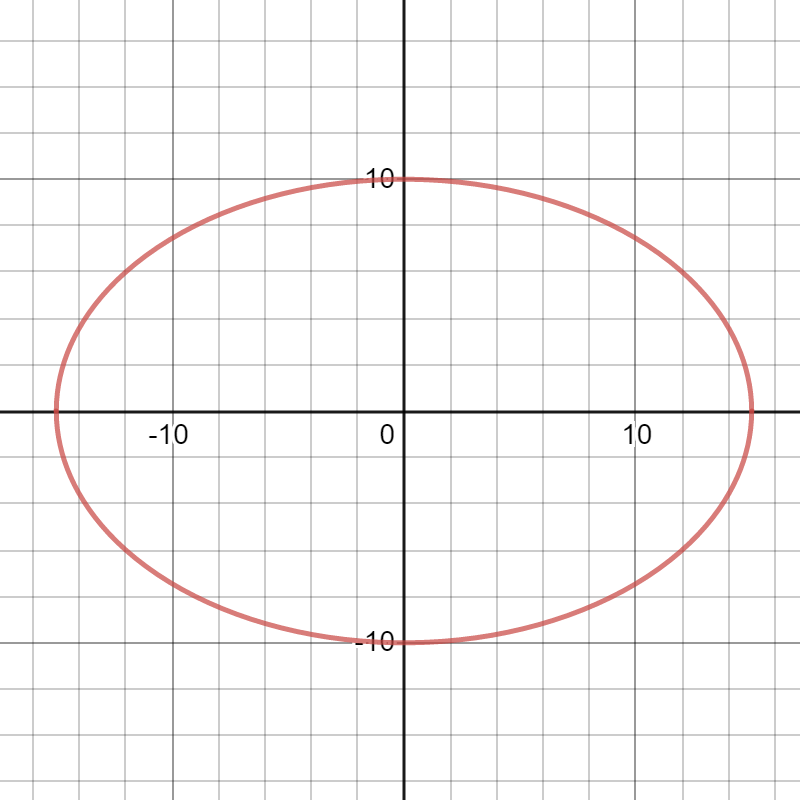
\includegraphics[scale=.3]{football.png}
        \caption{\textit{Visualization of ellipse bound by football}, also see embed below}
    \end{center}
\end{figure}
I found that the equation of an ellipse with a major axis of $30$ and minor axis of length $20$ is
\begin{equation}
    \frac{x^{2}}{15^{2}}+\frac{y^{2}}{10^{2}}=1
\end{equation}
Now to find the $A(x)$ function and try to integrate...
\begin{align}
    \intertext{First define area of equilateral triangles with respect to the base}
    A\left(b\right)                           & =\frac{b^{2}\sqrt{3}}{4}
    \intertext{Now we have to define the function of the ellipse in terms of $x$}
    \frac{x^{2}}{15^{2}}+\frac{y^{2}}{10^{2}} & =1                                                                                                                                                      \\
    \frac{y^{2}}{10^{2}}                      & =1-\frac{x^{2}}{15^{2}}                                                                                                                                 \\
    y^{2}                                     & =10^{2}\cdot\left(1-\frac{x^{2}}{15^{2}}\right)                                                                                                         \\
    y                                         & =\pm\sqrt{10^{2}\cdot\left(1-\frac{x^{2}}{15^{2}}\right)}
    \intertext{In this case, since we know that in an ellipse the $\pm$ portions provide an equal amount of height, we can just simplify that to $2$}
    y                                         & =2\sqrt{10^{2}\cdot\left(1-\frac{x^{2}}{15^{2}}\right)}
    \intertext{The factors can then be distributed further}
    y                                         & =\boxed{\sqrt{400\cdot\left(1-\frac{x^{2}}{15^2}\right)}}
    \intertext{Now to plug this back into our area function to make it in terms of $x$}
    A\left(b\right)                           & =\frac{b^{2}\sqrt{3}}{4}                                                                                                                                \\
    A(x)                                      & =\frac{\left(\sqrt{400\cdot\left(1-\frac{x^{2}}{15^2}\right)}\right)^{2}\sqrt{3}}{4}                                                                    \\
                                              & =\boxed{100\sqrt{3}\left(1-\frac{x^{2}}{15^2}\right)}
    \intertext{Now to find the $a$ and $b$, consider the $\pm a_1$ value of the ellipse}
    a_1                                       & =15                                                                                                                                                     \\
    a                                         & =\boxed{-15}                                                                                                                                            \\
    b                                         & =\boxed{15}
    \intertext{Now we can just integrate the area function from these ranges}
    \int_{a}^{b}A\left(x\right)dx             & =\int_{-15}^{15}\left(100\sqrt{3}\left(1-\frac{x^{2}}{15^2}\right)\right)dx                                                                             \\
                                              & =100\sqrt{3}\int_{-15}^{15}\left(1-\frac{x^{2}}{15^2}\right)dx                                                                                          \\
                                              & =100\sqrt{3}\left(x-\frac{x^{3}}{3\cdot 15^2}\right)\Big|_{-15}^{15}                                                                                    \\
                                              & =100\sqrt{3}\left(\left(15\right)-\frac{\left(15\right)^{3}}{3\cdot 15^2}-\left(\left(-15\right)-\frac{\left(-15\right)^{3}}{3\cdot 15^2}\right)\right) \\
                                              & =100\sqrt{3}\left(15-\frac{15}{3}+15-\frac{15}{3}\right)                                                                                                \\
                                              & =100\sqrt{3}\left(30-\frac{3375}{675}-\frac{3375}{675}\right)                                                                                           \\
                                              & =100\sqrt{3}\left(30-10\right)                                                                                                                          \\
                                              & =100\sqrt{3}\left(20\right)                                                                                                                             \\
                                              & =2000\sqrt{3}                                                                                                                                           \\
    \intertext{This is our value for one side of the football, so to include the other side we just need to double the previous volume}
    2000\sqrt{3}\cdot 2                       & =4000\sqrt{3}                                                                                                                                           \\
                                              & \approx\boxed{6928.20cm^3}
\end{align}
\section{Conclusion}
Tom should stop pumping air into the ball as soon as the pump reads approximately $6928.20cm^3$.
\end{document}